% \documentclass[a4paper,14pt]{article}
% \usepackage[utf8]{inputenc}
% \usepackage[T2A,T1]{fontenc}
% \usepackage[utf8]{inputenc}
% \usepackage[russian]{babel}
% \usepackage{array}
% \usepackage{multirow}
% \usepackage{diagbox}
% \usepackage{fancyhdr, mathtools, bm, geometry, graphicx, subcaption}
% \geometry{left=5pt, top=10pt, bottom=10pt, right=5pt,includehead}
% \usepackage[inline]{enumitem}

% \begin{document}

% \begin{titlepage}
% \centering
% \large Министерство науки и высшего образования Российской Федерации
% Федеральное государственное автономное образовательное учреждение высшего образования \\«Национальный исследовательский университет ИТМО» \\Факультет программной инженерии и компьютерной техники\\
% \vspace*{\fill}
% \LARGE ЛАБОРАТОРНАЯ РАБОТА №6\\ПО ИНФОРМАТИКЕ\\<<Работа с системой компьютерной вёрстки \TeX>>\\
% \LARGE Вариант №34 \\
% \vspace{4cm}
% \begin{flushright}
% \normalsize Группа: P3112\\
% \normalsize Выполнил: Соколов Анатолий\\
% \normalsize Проверил: к.т.н., преподаватель Белозубов А.В.\\
% \end{flushright}
% \vspace*{\fill}

% \centering
% \large 2022 год

% \end{titlepage}
% \setcounter{page}{2}
\twocolumn
\par
 Решения задач из этого номера можно посылать не позднее $31$ мая $1973$ года по адресу: $11701$, Москва В-$71$, Ленинский проспект, $15$, издательство “Наука”, журнал “Квант”. После адреса на конверте напишите, решения каких задач ~ вы ~посылаете,~ например: ~“Задачник “Кванта”, М$196$, М$198$ или “…Ф$210$”. Решения задач по каждому из предметов (математике или физике), а также новые задачи просьба присылать в отдельных конвертах. Оригинальные задачи, предлагаемые для публикации этих задач (на конверте пометьте: “Задачник кванта”, новая задача по физике” или “…новая задача по математике”). Задачи из разных номеров журнала присылайте в конвертах.
 \par
Задачи повышенной трудности отмечены звездочкой. \par
После формулировки задачи мы обычно указываем, кто предложил нам эту задачу. Разумеется, не все эти задачи публикуются впервые.

\section*{Задачи \\ М196-М200; Ф208-Ф212}
% \section*{}

 \begin{enumerate}[label={М}{{\arabic*}}{.}, font=\bfseries, wide,  labelindent=0pt, noitemsep]
    \setcounter{enumi}{195}
    \item В окружности радиуса $1$ проведено \\ несколько хорд. Докажите, что если каждый диаметр пересекает не более $k$ хорд то сумма длин хорд меньше $\pi k$ 

    \begin{flushright}
        \textit{А. Т. Колотов}
    \end{flushright}
    
    \item В прямоугольную таблицу из $m$ строк и $n$ столбов записаны $mn$ произвольных положительных чисел. Найдем произведение чисел в каждом столбце и затем сумму $S$ всех $n$ таких произведений. Докажите, что если переставить числа в каждой строке в порядке возрастания, то сумма $S$ для новой таблицы будет не меньше, чем в первоначальной. (На рисунке $1$ приведен один пример ситуации, описанной в задаче; здесь $m = 3, n = 4$.) \par
    \begin{tabular}{ cc }   % top level tables, with 2 columns
$S = 84$ & $S = 132$ \\  
% leftmost table of the top level table
\begin{tabular}{ |c|c|c|c| } 
 \hline
 1 & 5 & 6 & 2\\
 \hline
 4 & 3 & 7 & 2\\
 \hline
 1 & 2 & 1 & 2\\
 \hline
  
 \hline
 4 & 30 & 42 & 8\\
 \hline
\end{tabular} &  % starting rightmost sub table
% table 2
\begin{tabular}{ |c|c|c|c| } 
 \hline
 1 & 5 & 6 & 2\\
 \hline
 2 & 3 & 4 & 7\\
 \hline
 1 & 1 & 2 & 2\\
 \hline
  
 \hline
 2 & 6 & 40 & 84\\
 \hline
\end{tabular} \\
\end{tabular} \\

Рис. 1
\newline

Решите эту задачу: \par
	а) для $m = n = 2$ (для таблицы $2*2$); \par
	б) для $m = 2$ и произвольного n (для таблицы из двух строк); \par
	в)* для любых натуральных $m$ и $n$. \par


    \item Дан параллелограмм $ABCD$. На прямых $AB$ и $BC$ выбраны точки соответственно $H$ и $K$ так, что треугольники $KAB$ и $HCB$ равнобедренные ($KA = AB$ и $HC = CD$; рис.2 ). Докажите, что треугольник $KDH$ - тоже равнобедренный. 
    
    \begin{flushright}
     \textit{В. Л. Гутенмахер}
    \end{flushright}
    
    \begin{center}
         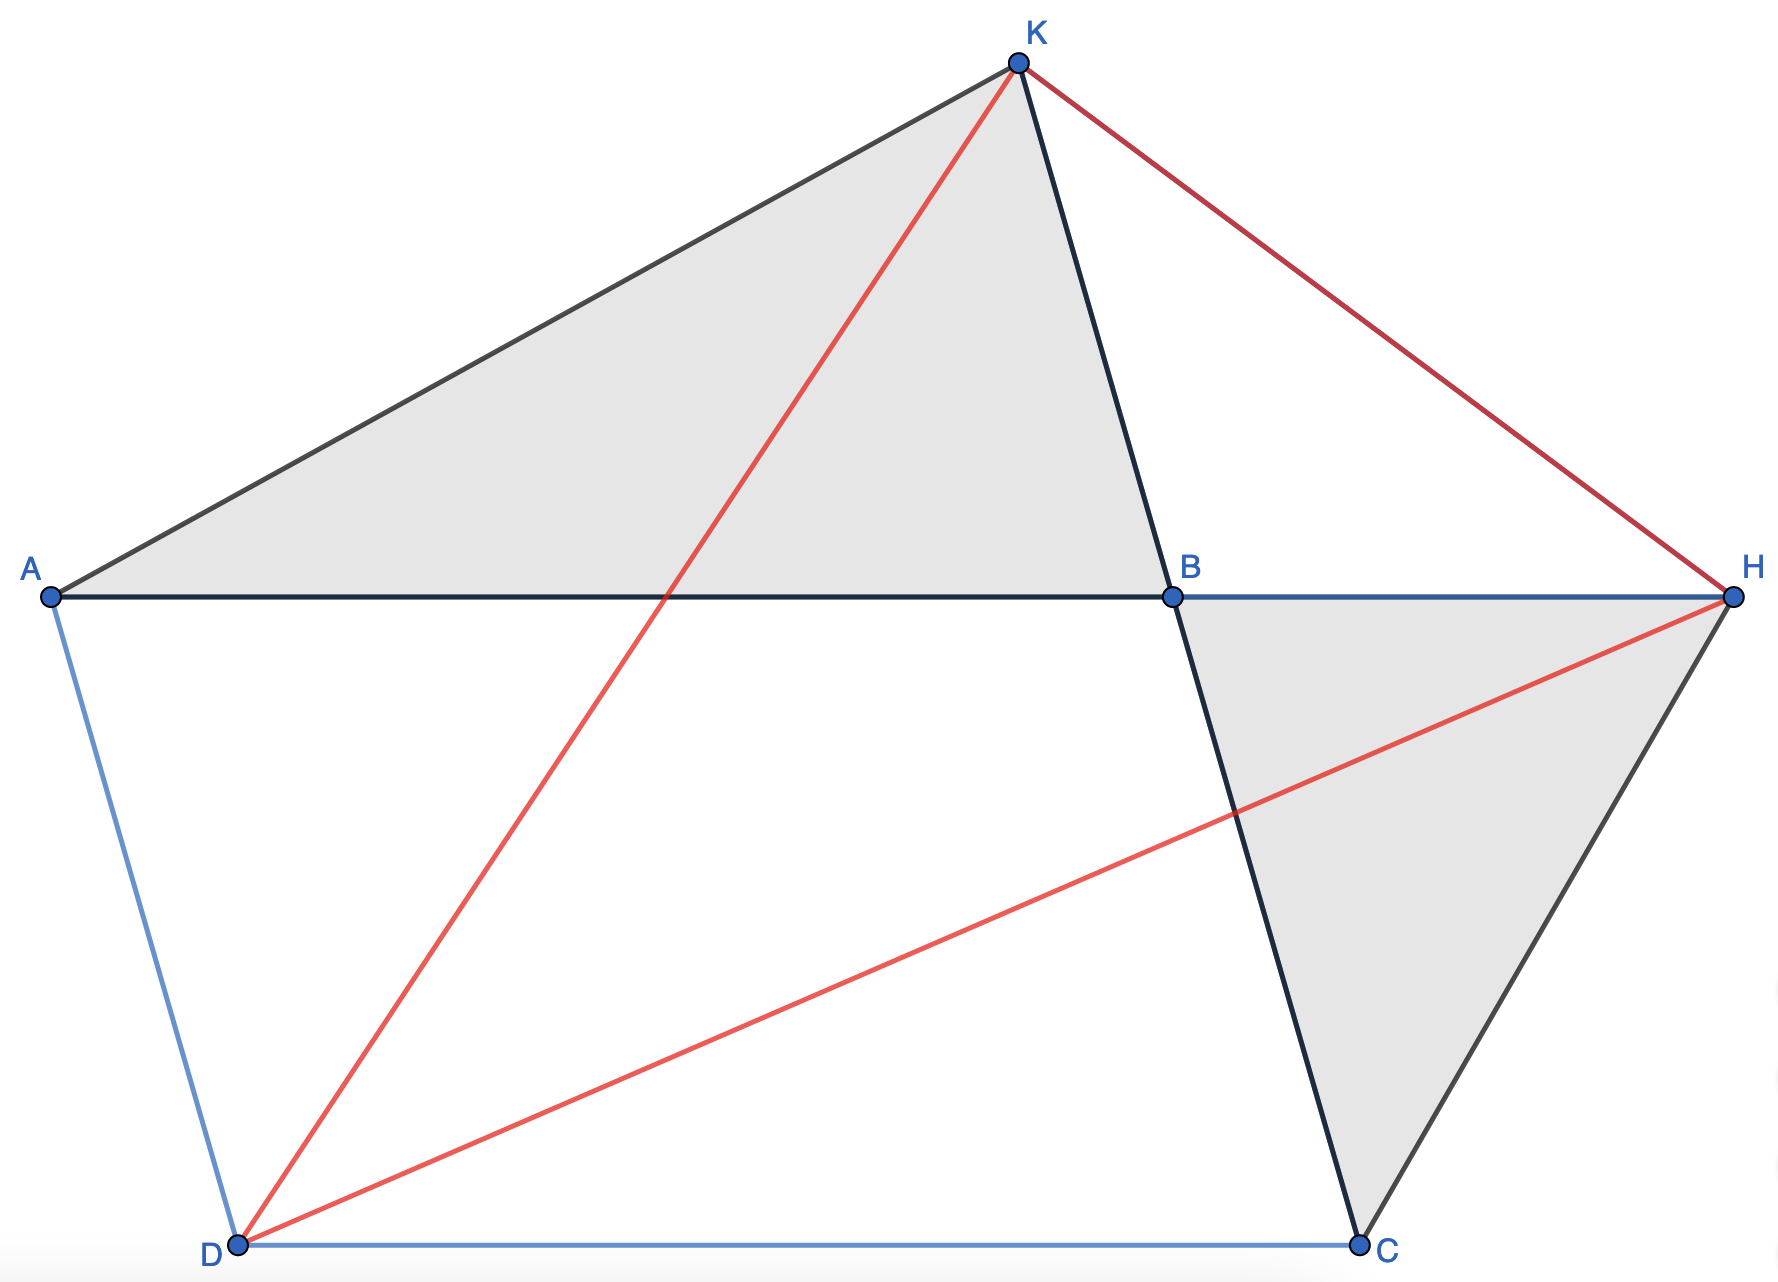
\includegraphics[width=160px]{polygon.png}
    \end{center}
   

Рис. 2
\newline
    \item а) Докажите, что сумма
    \begin{center}
    $C_{n}^{0} - C_{n}^{1} \frac{1}{4} + C_{n-2}^{2} \frac{1}{4^2} - ... + (-1)^i C_{n-i}^{i} \frac{1}{4^i}$
    \end{center}
    (сумма берется по всем целым $i$, $0 \leq i \leq \frac{n}{2}$) равна $\frac{n+1}{2^n}$ 
    \par
    б)* Докажите, что если $p$ и $q$ - различные числа и $p + q = 1$, то сумма 
    \begin{center}
    $C_{n}^{0}-C_{n-1}^{1}pq+C_{n-2}^{2}p^2q^2 - ... + (-1)^iC_{n-i}^{i}p^iq^i+...$
    \end{center}
    аналогичная предыдущей, равна $\frac{p^{n+1}-q^{n+1}}{p-q}$ \\
    при произвольном $n$. \par
    Здесь $C_{n}^{k}$ - биноминальные коэффициенты, то есть $C_{n}^{0} = 1$ и $C_{n}^{k} = \frac{n(n-1)...(n-k+1)}{1*2*...*k}$. О числах $C_{n}^{k}$ рассказывалось в «Кванте» №2 за этот год.) 
    \par

    \begin{flushright}
        \textit{Д. А. Фридкин}
    \end{flushright}
    
\item
    а) на рисунке 3 изображены шесть точек, которые лежат по три на четырех прямых. Докажите, что $24$ способами отобразить это множество из шести точек так, чтобы каждые три точки, лежащие на одной прямой, отображались в три точки, также лежащие на одной прямой. \par
    б) На рисунке 4 девять точек лежат по три на девяти прямых, причем через каждую точку проходит по три такхи прямых. Эти девять точек  и девять прямых образуют знаменитую “конфигурацию Паскаля”. Сколькими способами можно множество наших девяти точек отобразить на себя так, чтобы каждая тройка точек, лежащая на одной из девяти наших прямых, отображалась на тройку точек, которая тоже лежит на некоторой прямой на нашей конфигурации? \par
    в) Тот же вопрос для конфигурации Дезарга (из десяти точек и десяти прямых), изображенной на рисунке 5.
     
    \begin{flushright}
        \textit{А. Н. Колмогоров}
    \end{flushright}
\end{enumerate}    
 \begin{enumerate}[label={Ф}{{\arabic*}}{.}, font=\bfseries, wide,  labelindent=0pt, noitemsep]
\setcounter{enumi}{207}
    \item
    У автомобиля, участвующего в гонке, лопается шина. Оценить, с какой скоростью должен ехать автомобиль, чтобы шина не сминалась.
    
    \begin{flushright}
        \textit{П. Л. Капица}
    \end{flushright}
    
    \item
    Смоделировать траекторию заряженной частицы в магнитном поле можно, поместив в однородное магнитное поле закрепленный на концах гибкий проводник, по которому пропускается ток. Каким будет натяжение такого провода при токе 1 а, если он имитирует
    \begin{center}
         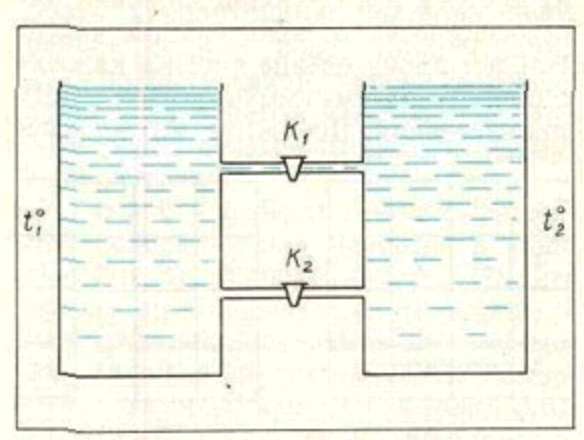
\includegraphics[width=190px]{pic6.png}
    \end{center}
    Рис. 6
    \newline
\end{enumerate}    

 
% \addtocounter{figure}{1}

% \begin{figure}
% \centering
% \begin{minipage}{.25\textwidth}
%   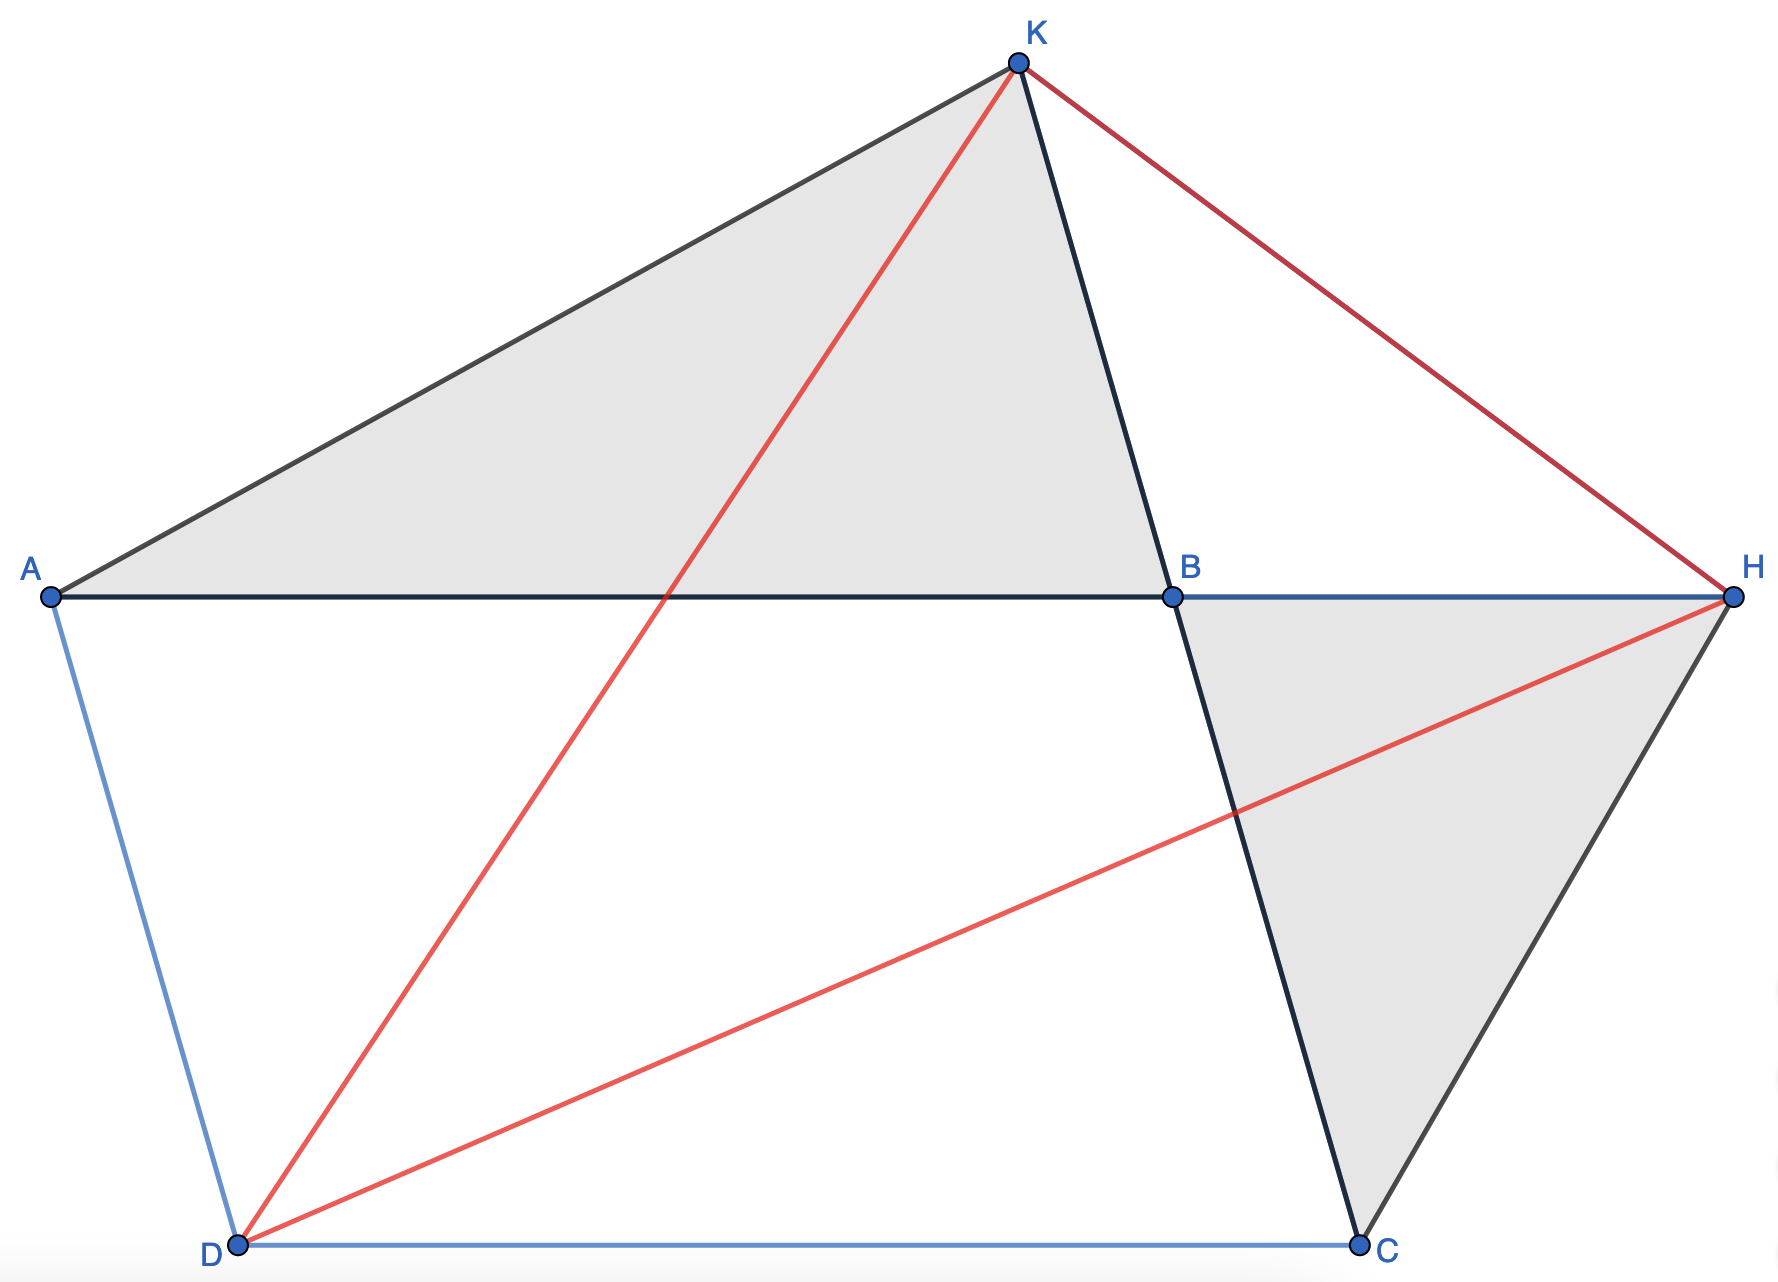
\includegraphics[width=\linewidth]{polygon.png}
% \captionof{figure}{}
% \end{minipage}

% \end{figure}



% \begin{tabular}{ |p{0.5cm} |p{0.5cm}|p{0.5cm}|p{0.5cm}|  }
% %  \multicolumn{4}{|c|}{tets} \\
%  \hline
%  1 & 5 & 6 & 2\\
%  \hline
%  4 & 3 & 7 & 2\\
%  \hline
%  1 & 2 & 1 & 2\\
%  \hline
  
%  \hline
%  4 & 30 & 42 & 8\\
%  \hline
% \end{tabular}



% \begin{tabular}{ |p{0.5cm} |p{0.5cm}|p{0.5cm}|p{0.5cm}|  }
% %  \multicolumn{4}{|c|}{tets} \\
%  \hline
%  1 & 5 & 6 & 2\\
%  \hline
%  2 & 3 & 4 & 7\\
%  \hline
%  1 & 1 & 2 & 2\\
%  \hline
  
%  \hline
%  2 & 6 & 40 & 84\\
%  \hline
% \end{tabular}

% \begin{table}[h]
%   \centering
%  \captionsetup{format=plain,font=it}
%     \caption{}
% \begin{tabular}{ r | c | c | c | c | c | c | c | c | c | c | c }
%  А&*&*&*&*&*&*&*&*&*&М \\ \hline
%  А&*&*&*&*&*&*&*&*&*&Т \\ \hline
%  Е&*&*&*&*&*&*&*&*&*&Т \\ \hline
%  И&*&*&*&*&*&*&*&*&*&Л \\ \hline

% \end{tabular}

% \end{table}


% \end{document}
